\section{WP3 Tasks: Summary of Contribution}
\label{sec:tasks}

\subsection{T3.1 Community Management}

Task 3.1 works in close cooperation with WP5 to explore community management, which is reflected in the diverse CIVIS platform design supporting social sharing, housing cooperative activities in the Swedish test site and the two local consortia in the Italian test site respectively tailored to the local context. Sec.~\ref{sec:design} discussed the design in detail, which includes:   

\begin{itemize}
\item The design of YouPower supports housing cooperatives in energy management and more specifically in taking cooperative energy reduction actions. It also allows comparison between cooperatives based on each cooperative's energy performance. 

\item The design of YouPower facilitates the engagement of all household members for pro-enviromental energy actions. 

\item The openness of energy data (with user permission) and the comparative visualization  at community level is key to facilitate users in sharing experience for taking energy reduction and load-shifting actions collectively. 

\item The design of YouPower provides features that support social sharing and knowledge exchange, and use social norms and public commitment to promote environmental energy actions. 

\item The design of YouPower supports intrinsic motivations as well as active and volitional forms of extrinsic motivation such as environmental values and social belongingness and relatedness. 
\end{itemize}

\subsection{T3.2 Energy Consumer Profiling}

This task was carried out between the last quarter of 2014 and the first quarter of 2015.
The goal was to provide a method to process individual electricity consumption
data in order to define a set of features that can characterize the behavioral patterns of each
consumer, and a way to group similar consumers together. The process devised can be summarized
as follows:

\begin{enumerate} 
\item Energy data is provided in XML format in the green button standard.

\item Energy data is stored into a MongoDB database.

\item The data is cleaned. In particular, missing data are detected and, where possible, interpolated. Outliers are detected and substituted with interpolated data. A report with all the modifications performed on
data is produced. 

\item Features are extracted from each individual energy consumption dataset. Examples of such
features are: average daily consumption, average hourly consumption, peak consumption, peak hour
consumption, total daily consumption. Each electric energy consumption time series is mapped to a
tuple of such features and stored in a MongoDB database.

\item Features tuples are clustered into similar groups. A range of algorithms are provided. These
algorithms are available in the scientific computing package \textit{scikit-learn}\footnote{\url{http://scikit-learn.org}}. Examples of those algorithms are K-means,
hierarchical clustering, affinity propagation, spectral clustering, DB scan.

\item A set of metrics to evaluate the goodness of the achieved clustering is provided. These metrics are implemented by scikit-learn. Examples of those are 
DBI (Davies-Bouldin Index),
CDI  (Cluster Dispersion Indicator),
MDI (Modified Dunn Index),
MSE (Mean Squared Error).
\end{enumerate}

The software is written in Python and it is available at the GitHub repository\footnote{\url{https://github.com/CIVIS-project/Consumer_profiling}}.

Note: after discussing with the CIVIS partners, we agreed that given the test site context of CIVIS, the consumption profiling part was not a most promising path towards load-shifting. Hence, although significant work has been done in this direction, we did not integrate this contribution to the YouPower application. (Nonetheless this contribution can still be useful for others.)
Instead, we devoted extra time and effort for the design and development of an energy production forecasting
system, Sec.~\ref{sec:energydata}, which can have a strong impact to help users achieve the load-shifting goals.

\subsection{T3.3 Interface with System Level}

The task 3.3 of CIVIS WP3 took care of exploring the different models for interconnecting the system level developed in WP4, the Energy ICT Platform, with the user level subsystem developed in WP3.

This work, performed between T02 and T08 of CIVIS project, was strictly in connection with the one performed in D4.3, where the interconnection of the two subsystems has been implemented and has been documented in D4.1, where the different models of interconnection have been described.

Sec. 8.3 of CIVIS D4.1 contains the descriptions of three different models that could be used in order to implement the connection between User Level and System Level:

\begin{itemize}
\item Solution 1: single connection and native HiReply MS SQL DB (Sec. 8.3.1 of D4.1);
\item Solution 2: single connection and use of a remote DB (Sec. 8.3.2 of D4.1);
\item Solution 3: double connection and use of a remote DB (Sec. 8.3.3 of D4.1).
\end{itemize}

Sec. 8.3 of D4.1 also describes the different features, in terms of scalability, that the three solutions can provide. For the deployment of CIVIS ICT Platform we adopted Solution 1, because it was suitable for achieving all the fixed goals in the provided project time frame and that is represented in Figure \ref{fig:wp4}.

\begin{figure}[h!]
\begin{center}
	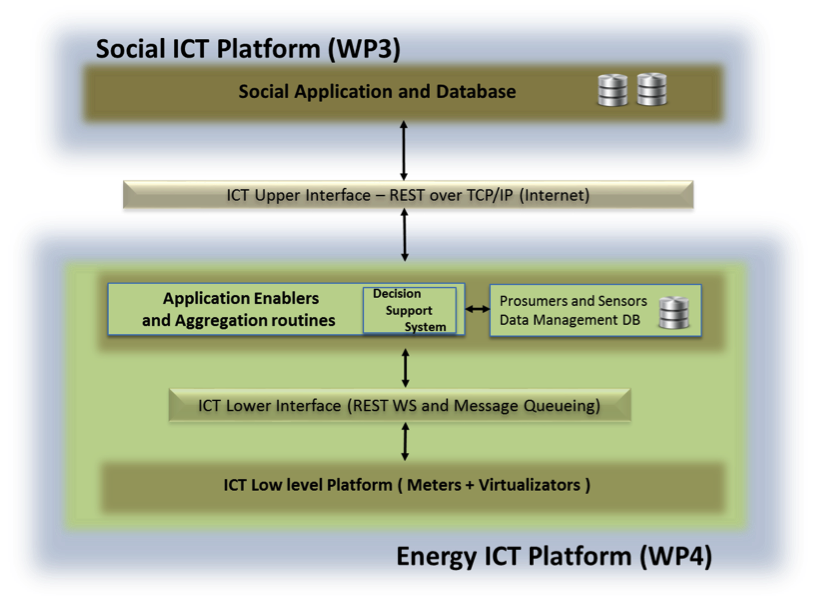
\includegraphics[width=.85\textwidth]{img/wp4.png}
	\caption{Solution 1 implemented in the CIVIS deployment}\label{fig:wp4}
\end{center}
\end{figure}

The usage of a SQL database, already integrated into the HiReply Platform, simplified the configuration and maintenance operations associated to the system database, without presenting those problems that could be present in large pilot site deployments with SQL technologies.
The solution 1 foresaw only one communication channel between user and system level architectures. For this reason the interface developed in WP4 reflects this schema and implements all the communication APIs on the same server.
The implemented APIs, documented in Sec. 5.9 of D4.3 v2.0, provide the possibility to retrieve, from the Energy ICT Platform developed in WP4, the following information:

\begin{itemize}
\item Energy data coming from DSOs and CIVIS additional sensors, provided in GreenButton format, suitably extended for introducing some parameters useful for CIVIS applications;
\item Non-energy information such as the list of all usage points monitored in the system, weather info, the list of the recognized events associated to a usage point in a certain period, etc. 
\end{itemize}

\subsection{T3.4 Energy Service Context}

This section highlights the lessons learned of business models for emerging social energy initiatives.
In its final deliverable (D6.3) WP6 concludes with four main types of business models that can be applied to the CIVIS maturity scheme (depicting the development from emerging and promising to established energy initiative). 

\begin{itemize}
\item Efficiency Effects: becoming better at what you're doing - activities that enhance brand awareness and increase customer engagement.
\item Diversification: introducing products and services that are different that the initial domain of the organisation -- for (indirect) social as well as (longer term) financial benefits. 
\item Service Provisioning: facilitating others with available expertise -- providing available services at marginal costs to others.
\item Incubation: enabling innovation outside the organisation -- high(er) risk investment in the hope to achieve a financial or technical return on investment. 
\end{itemize}

Regardless of the specific maturity stage an organisation stage has achieved, of these four business model types, trying to achieve efficiency effects is one that is most applicable to any maturity stage. 
% 
To that effect, the mobile energy app that has been developed as part of this work package can be placed in this category. It is an example of activities that enhance brand awareness and increase customer engagement in order to either make the members of the cooperatives more energy aware (and efficient) or that it convinces more inhabitants to join the cooperative.

As such, these developments are (when introduced in the right way) powerful tools that can strengthen a chosen business model. In work package 6 much attention has given to a step-by-step approach for (emerging) energy initiatives and particularly the use of tooling such as the business model canvas (bmc). The developed tools in WP3 provides a solution for cooperatives to properly address their (mobile and online) members -- in other words, describing the ``channel'' element of the bmc.

Examples of this have become apparent in surveys with the board members of the testsites
in Sweden and Italy. What CIVIS learned is that there is a distinct advantage in having
a collaboration or information application available to the cooperative members.
While it does not come as a surprise that providing members with information on energy
generation, consumption and saving does increases awareness ? it is the extent of the impact
on awareness that interests us.

While initial uptake of the CIVIS apps has been slow, once people started to use it the
awareness of what is happening within the cooperative as a whole is certainly increasing.
Throughout the past months, several board members have noticed increased feedback from members since making the mobile apps available. For leadership, this kind of feedback
and interaction is particularly helpful terms of gauging if certain initiatives have a positive
effect within the cooperation. In a sense this contributes more to their understanding than
just looking at the amount of website ``hits'' that are available through the IT responsible
department or person. 

